%  template.tex for Biometrics papers
%
%  This file provides a template for Biometrics authors.  Use this
%  template as the starting point for creating your manuscript document.
%  See the file biomsample.tex for an example of a full-blown manuscript.

%  ALWAYS USE THE referee OPTION WITH PAPERS SUBMITTED TO BIOMETRICS!!!
%  You can see what your paper would look like typeset by removing
%  the referee option.  Because the typeset version will be in two
%  columns, however, some of your equations may be too long. DO NOT
%  use the \longequation option discussed in the user guide!!!  This option
%  is reserved ONLY for equations that are impossible to split across 
%  multiple lines; e.g., a very wide matrix.  Instead, type your equations 
%  so that they stay in one column and are split across several lines, 
%  as are almost all equations in the journal.  Use a recent version of the
%  journal as a guide. 
%  
\documentclass[useAMS,referee]{biom}

%documentclass[useAMS]{biom}
%
%  If your system does not have the AMS fonts version 2.0 installed, then
%  remove the useAMS option.
%
%  useAMS allows you to obtain upright Greek characters.
%  e.g. \umu, \upi etc.  See the section on "Upright Greek characters" in
%  this guide for further information.
%
%  If you are using AMS 2.0 fonts, bold math letters/symbols are available
%  at a larger range of sizes for NFSS release 1 and 2 (using \boldmath or
%  preferably \bmath).
% 
%  Other options are described in the user guide. Here are a few:
% 
%  -  If you use Patrick Daly's natbib  to cross-reference your 
%     bibliography entries, use the usenatbib option
%  -  If you use \includegraphics (graphicx package) for importing graphics
%     into your figures, use the usegraphicx option
% 
%  If you wish to typeset the paper in Times font (if you do not have the
%  PostScript Type 1 Computer Modern fonts you will need to do this to get
%  smoother fonts in a PDF file) then uncomment the next line
%  \usepackage{Times}

%%%%% PLACE YOUR OWN MACROS HERE %%%%%

\def\bSig\mathbf{\Sigma}
\newcommand{\VS}{V\&S}
\newcommand{\tr}{\mbox{tr}}

%  The rotating package allows you to have tables displayed in landscape
%  mode.  The rotating package is NOT included in this distribution, but
%  can be obtained from the CTAN archive.  USE OF LANDSCAPE TABLES IS
%  STRONGLY DISCOURAGED -- create landscape tables only as a last resort if
%  you see no other way to display the information.  If you do do this,
%  then you need the following command.

%\usepackage[figuresright]{rotating}
\usepackage[labelfont=bf]{caption}

%%%%%%%%%%%%%%%%%%%%%%%%%%%%%%%%%%%%%%%%%%%%%%%%%%%%%%%%%%%%%%%%%%%%%

%  Here, place your title and author information.  Note that in 
%  use of the \author command, you create your own footnotes.  Follow
%  the examples below in creating your author and affiliation information.
%  Also consult a recent issue of the journal for examples of formatting.

\title[Visualization methods for RNA-sequencing data analysis]{Visualization methods for RNA-sequencing data analysis}

%  Here are examples of different configurations of author/affiliation
%  displays.  According to the Biometrics style, in some instances,
%  the convention is to have superscript *, **, etc footnotes to indicate 
%  which of multiple email addresses belong to which author.  In this case,
%  use the \email{ } command to produce the emails in the display.

%  In other cases, such as a single author or two authors from 
%  different institutions, there should be no footnoting.  Here, use
%  the \emailx{ } command instead. 

%  The examples below corrspond to almost every possible configuration
%  of authors and may be used as a guide.  For other configurations, consult
%  a recent issue of the the journal.

%  Single author -- USE \emailx{ } here so that no asterisk footnoting
%  for the email address will be produced.

%\author{John Author\emailx{email@address.edu} \\
%Department of Statistics, University of Warwick, Coventry CV4 7AL, U.K.}

%  Two authors from the same institution, with both emails -- use
%  \email{ } here to produce the asterisk footnoting for each email address

%\author{John Author$^{*}$\email{author@address.edu} and
%Kathy Authoress$^{**}$\email{email2@address.edu} \\
%Department of Statistics, University of Warwick, Coventry CV4 7AL, U.K.}

%  Exactly two authors from different institutions, with both emails  
%  USE \emailx{ } here so that no asterisk footnoting for the email address
%  is produced.

%  Three or more authors from same institution with all emails displayed
%  and footnoted using asterisks -- use \email{ } 

%\author{John Author$^*$\email{author@address.edu}, 
%Jane Author$^{**}$\email{jane@address.edu}, and 
%Dick Author$^{***}$\email{dick@address.edu} \\
%Department of Statistics, University of Warwick, Coventry CV4 7AL, U.K}

%  Three or more authors from same institution with one corresponding email
%  displayed

%\author{John Author$^*$\email{author@address.edu}, 
%Jane Author, and Dick Author \\
%Department of Statistics, University of Warwick, Coventry CV4 7AL, U.K}

%  Three or more authors, with at least two different institutions,
%  more than one email displayed 

\author{Lindsay Rutter$^{1,*}$\email{lrutter@iastate.edu} and 
Dianne Cook$^{2,**}$\email{dicook@monash.edu} \\
$^{1}$Bioinformatics and Computational Biology Program, Iowa State University, Ames, Iowa, U.S.A \\
$^{2}$Department of Department of Econometrics and Business Statistics, Monash University, Clayton, Australia}

%  Three or more authors with at least two different institutions and only
%  one email displayed

%\author{John Author$^{1,*}$\email{author@address.edu}, 
%Wilma Flinstone$^{2}$, and Barney Rubble$^{2}$ \\
%$^{1}$Department of Statistics, University of Warwick, Coventry CV4 7AL, U.K \\
%$^{2}$Department of Geology, University of Bedrock, Bedrock, Kansas, U.S.A.}

\usepackage{graphicx}
\begin{document}


%  This will produce the submission and review information that appears
%  right after the reference section.  Of course, it will be unknown when
%  you submit your paper, so you can either leave this out or put in 
%  sample dates (these will have no effect on the fate of your paper in the
%  review process!)

%  These options will count the number of pages and provide volume
%  and date information in the upper left hand corner of the top of the 
%  first page as in published papers.  The \pagerange command will only
%  work if you place the command \label{firstpage} near the beginning
%  of the document and \label{lastpage} at the end of the document, as we
%  have done in this template.

%  Again, putting a volume number and date is for your own amusement and
%  has no bearing on what actually happens to your paper!  

%  The \doi command is where the DOI for your paper would be placed should it
%  be published.  Again, if you make one up and stick it here, it means 
%  nothing!

%  This label and the label ``lastpage'' are used by the \pagerange
%  command above to give the page range for the article.  You may have 
%  to process the document twice to get this to match up with what you 
%  expect.  When using the referee option, this will not count the pages
%  with tables and figures.  

\label{firstpage}

%  put the summary for your paper here

\begin{abstract}

It was initially claimed that RNA-seq produced unbiased data that did not require sophisticated normalization. However, studies have since revealed that RNA-seq data is biased and that accurate detection of differentially expressed genes is not a trivial task. In light of these findings, researchers should analyze RNA-seq data like they would any other biased multivariate data. The most effective approach to modern data analysis is to iterate between models and visuals, and to enhance the appropriateness of models based on feedback from visuals. Unfortunately, researchers do not often use models and visuals in a complimentary fashion when analyzing RNA-seq data. Here, we use real RNA-seq data to show that our visualization tools can detect normalization problems, DEG designation problems, and common errors in RNA-seq analysis. We also show that our tools can identify genes of interest that cannot be obtained by models. In this paper, we do not propose that users radically change their approach to RNA-seq analysis. Instead, we propose that users simply modify their approach to RNA-seq analysis by assessing the sensibility of their models with multivariate statistical graphics.

\end{abstract}

%  Please place your key words in alphabetical order, separated
%  by semicolons, with the first letter of the first word capitalized,
%  and a period at the end of the list.
%

\begin{keywords}

Data visualization; Exploratory data analysis; Interactive graphics; RNA-sequencing; Statistical graphics

\end{keywords}

%Data visualization; Exploratory data analysis; Interactive graphics; RNA-sequencing


%  As usual, the \maketitle command creates the title and author/affiliations
%  display 

\maketitle

%  If you are using the referee option, a new page, numbered page 1, will
%  start after the summary and keywords.  The page numbers thus count the
%  number of pages of your manuscript in the preferred submission style.
%  Remember, ``Normally, regular papers exceeding 25 pages and Reader Reaction 
%  papers exceeding 12 pages in (the preferred style) will be returned to 
%  the authors without review. The page limit includes acknowledgements, 
%  references, and appendices, but not tables and figures. The page count does 
%  not include the title page and abstract. A maximum of six (6) tables or 
%  figures combined is often required.''

%  You may now place the substance of your manuscript here.  Please use
%  the \section, \subsection, etc commands as described in the user guide.
%  Please use \label and \ref commands to cross-reference sections, equations,
%  tables, figures, etc.
%
%  Please DO NOT attempt to reformat the style of equation numbering!
%  For that matter, please do not attempt to redefine anything!


\section{Introduction}
\label{s:Introduction}

RNA-sequencing (RNA-seq) uses next-generation sequencing (NGS) to estimate the quantity of RNA in biological samples at given timepoints. In recent years, decreasing cost and increasing throughput has rendered RNA-seq an attractive alternative to transcriptome profiling. Prior to RNA-seq, gene expression studies were performed with microarray techniques, which required prior knowledge of reference sequences. RNA-seq does not have this limitation, and has enabled a new range of applications such as transcriptome de novo assembly (Robertson et al., 2010) and detection of alternative splicing processes (Anders, Reyes, and Huber, 2012; Pan et al., 2008). Coupled with its high resolution and sensitivity, RNA-seq will likely revolutionize our understanding of the intricacies of eukaryotic transcriptomes (Wang, Gerstein, and Snyder, 2009; Zhao et al., 2014).

RNA-seq data is multivariate data, and its basic form is a matrix containing mapped read counts for \textit{n} rows of genes and \textit{p} columns of samples. These mapped read counts provide estimations of the gene expression levels across samples. Researchers typically conduct RNA-seq studies to identify differentially expressed genes (DEGs) between treatment groups. In most popular RNA-seq analysis packages, this objective is approached with models, such as the negative binomial model (Anders and Huber, 2010; Trapnell et al., 2013; Trapnell et al., 2012; Robinson et al., 2010) and linear regression models (Law et al., 2014).

Initially, it was widely claimed that RNA-seq produced unbiased data that did not require sophisticated normalization (Wang et al., 2009; Morin et al., 2008; Marioni et al., 2008). However, numerous studies have since revealed that RNA-seq data is replete with biases and that accurate detection of DEGs is not a negligible task. Problems that complicate the analysis of RNA-seq data include nucleotide and read-position biases (Hansen et al., 2010), biases related to gene lengths and sequencing depths (Oshlack, Robinson, and Young, 2010; Robinson and Oshlack, 2010), biases introduced during library preparation (McIntyre et al., 2011), biases pertaining to the number of replications (Schurch et al., 2016), biases derived from overlapping sense-antisense transcripts and gene isoforms (Trapnell et al., 2013), and the confounding combination of technical and biological variability (Bullard et al., 2010).

In light of these complications, researchers should analyze RNA-seq data like they would any other biased multivariate data. Simply applying models to such data is problematic because models hold assumptions that they alone cannot call into question. Fortunately, data visualization enables researchers to see patterns and problems they may not otherwise detect with traditional modeling. As a result, the most effective approach to data analysis is to iterate between models and visuals, and enhance the appropriateness of applied models based on feedback from visuals (Shneiderman, 2002). With RNA-seq data, we primarily want to compare the variability between replicates and between treatment groups. This is visually best achieved by drawing the mapped read count distributions across all genes and samples. Unfortunately, the few plotting tools offered in popular RNA-seq packages do not allow users to effectively view their data in this manner.

In this paper, we strive to remedy this problem by publishing new and effective RNA-seq plotting tools. We use real RNA-seq data to show that our tools can detect normalization problems, DEG designation problems, and common errors in the analysis pipeline. We also show that our tools can identify genes of interest that cannot otherwise be obtained by models. We emphasize that interactive graphics should be an indisposable component of modern RNA-seq analysis: Researchers should be able to quickly flip through plots of genes that appear promising or problematic, and link between plots to swiftly obtain various perspectives of their data. Here, we do not propose that users drastically change their approach to RNA-seq analysis. Instead, we propose that users simply modify their approach to RNA-seq analysis by assessing the sensibility of their models with multivariate graphical tools, namely with parallel coordinate plots, scatterplot matrices, and replicate point plots.

\section{Parallel Coordinate Plots}
\label{s:Parallel Coordinate Plots}

Parallel coordinate plots are essential to visually verify the relationships between variables in multivariate data. A parallel coordinate plot draws each row (gene) as a line. Connections between samples with positive correlations are flat, and connections between samples with negative correlations are crossed. The ideal dataset has more variability between treatments than between replicates. Researchers can quickly confirm this with a parallel coordinate plot: There should be flat connections between replicates but crossed connections between treatments.

There are several packages within the Bioconductor software that provide graphics for RNA-seq data analysis (Huber et al., 2015). Two of the most common graphic techniques are side-by-side boxplots and Multidimensional Scaling (MDS) plots (Love, Huber, and Anders, 2014; Risso et al., 2011; Robinson et al., 2010; Su et al., 2016; Ritchie et al., 2015; Marini, 2017). Unfortunately, these plots can hide problems that still exist in the data even after normalization and that could be better detected with parallel coordinate plots.

Figure~\ref{2group} exemplifies this problem for two simulated datasets, one displayed on the left half and the other displayed on the right half of the figure. Each dataset contains two treatment groups (A and B) with three replicate samples. We cannot detect any notable differences between the left and right datasets from the side-by-side boxplots at the top of the figure as they both show fairly consistent five number summaries across their six samples. Likewise, we cannot detect notable differences between the datasets from the MDS plots in the middle of the figure as they both suggest that the datasets are clustered by the two treatment groups, although the first replicate from treatment A appears as an outlier in the right MDS plot.

\begin{figure}[t!]
\begin{center}
\centerline{\fbox{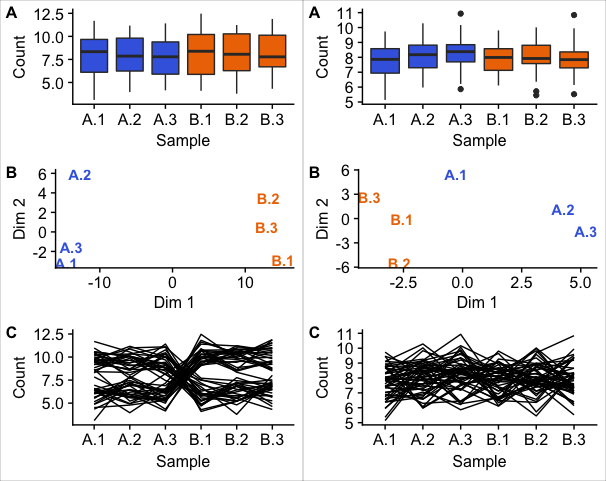
\includegraphics[width=7.5cm]{/Users/lindz/JDSPaper/Bioinformatics/Pictures/bmp/Color/2group.png}}}
\end{center}
\caption{One simulated dataset is shown on the left half and another simulated dataset is shown on the right half of the figure. We do not see crucial distinctions between the left and right datasets when we compare their boxplots (A subplots) and MDS plots (B subplots). However, their parallel coordinate plots (C subplots) show a critical difference between their structures. Namely, the left dataset is composed of genes with small replicate variation and large treatment group variation (suggesting DEGs), while the right dataset is composed of genes with similar variation between replicates and treatment groups (not suggesting DEGs). 
\label{2group}}
\end{figure}

Despite this, we immediately see from the parallel coordinate plots on the bottom of the figure that the left and right datasets have an important difference. The left dataset has consistent (level) lines between replicates and inconsistent (crossed) lines between treatment groups. This suggests that some of the genes (lines) have consistently low values for treatment group A and consistently high values for treatment group B, while some genes have the opposite phenomenon. As a result, these plotted genes are likely candidates for differential expression. In contrast, the right dataset does not possess this ideal structure and suggests that the genes may not be candidates for differential expression. We could not see this important distinction from the side-by-side boxplots and MDS plots because they simply provide summaries about the data at the sample resolution, while the parallel coordinate plot shows the sample connections for each of the 50 genes.

\section{Scatterplot matrices}
\label{s:Scatterplot matrices}

\subsection{Overview of scatterplot matrices}
\label{s:Overview of scatterplot matrices}

A scatterplot matrix is another effective multivariate visualization tool that plots the mapped read count distributions across all genes and samples. Specifically, it represents each row (gene) as a point in each scatterplot. With this method, users can quickly discover unexpected patterns, recognize geometric shapes, and assess the structure and association between multiple variables in a manner that is different from most common practices. 

The ideal dataset will have larger variability between treatment groups than between replicates. As Figure~\ref{cotyIdeal} shows, researchers can quickly confirm this with a scatterplot matrix. Within each scatterplot, most genes should fall along the \textit{x=y} line (in red) as we expect only a small proportion of them to show differential expression between samples. However, a fraction of the genes should have lower variability between replicates than between treatments, and so we should expect the spread of the scatterplot points to fall more closely along the \textit{x=y} relationship between replicates than between treatments. Indeed, in Figure~\ref{cotyIdeal}, we created a scatterplot matrix for a public RNA-seq dataset that contains three replicates for two developmental stages of soybean cotyledon (S1 and S2) (Brown and Kudson, 2015). We can immediately verify that the nine scatterplots between treatment pairs (in the bottom-left corner of the matrix) have more spread around the \textit{x=y} line than the six scatterplots between replicate pairs.

\begin{figure}
\begin{center}
\centerline{\fbox{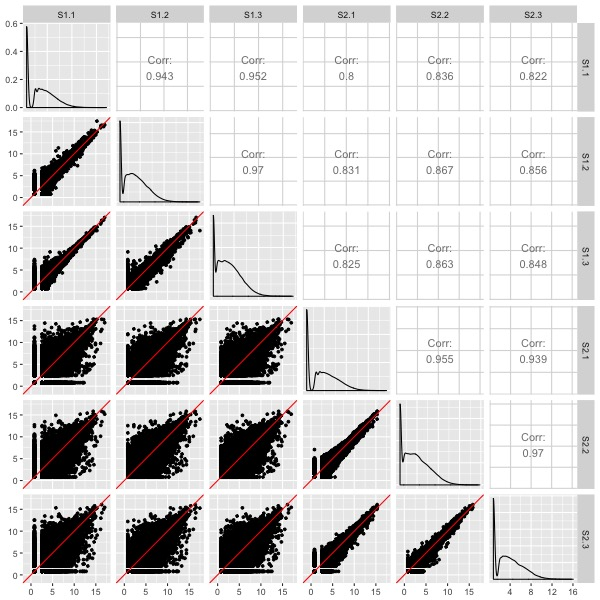
\includegraphics[width=7.5cm]{/Users/lindz/JDSPaper/Bioinformatics/Pictures/SwitchSample/Switch12/NotSwitch/S1_S2_points_size1.jpg}}}
\end{center}
\caption{Example of the expected structure of an RNA-seq dataset. Within a given scatterplot, most genes (points) should fall along the \textit{x=y} line. We should see genes deviate more strongly from the \textit{x=y} line in treatment scatterplots than in replicate scatterplots.
\label{cotyIdeal}}
\end{figure}

After confirming this expected trend, users can use the scatterplot matrix to focus on subsets of genes: Outlier genes that deviate from the \textit{x=y} line in replicate scatterplots might be problematic, whereas outlier genes that deviate from the \textit{x=y} line in treatment scatterplots might be DEGs. In order to achieve this functionality, the plots must be rendered interactive.

Notice that each gene in our data is plotted once in each of the 15 scatterplots. With 73,320 genes in our data, more than one million points must be plotted. Rendering all points interactive would slow down the interactive capabilities of the plot. To solve this, we can tailor the geometric object of the scatterplots to be hexagon bins rather than points. This dramatically reduces the number of geometric objects to be plotted, and increases the interactivity speed.

The reader can visit https://rnaseqvisualization.shinyapps.io/scatmat to access the interactive version of Figure~\ref{cotyIdeal}. Readers can read the ``About" Tab to fully understand how to use the application. Essentially, the user can hover over a hexagon bin to see how many genes it contains. When the user clicks on a hexagon bin, the names of the genes are listed and superimposed as orange points across all scatterplots. The genes are also linked to a second plot that superimposes them as parallel coordinate lines on a side-by-side boxplot of all gene counts. This interactivity and linking allows users to quickly examine genes of interest from multiple perspectives superimposed onto the summary of all genes in the dataset. 

The scatterplot matrix can also be used after DEG calls to quickly examine DEGs obtained from a given model. As shown in Figure~\ref{scatPCP}, the DEGs can be superimposed as orange points onto the scatterplot matrix. We expect for DEGs to fall along the \textit{x=y} line for replicates and deviate from the \textit{x=y} line between treatment groups, as is confirmed in Figure~\ref{scatPCP}. As a side note, we can also link these DEGs as parallel coordinate lines on a side-by-side boxplot like in Figure~\ref{scatPCP} to confirm the expected pattern of differential expression from a second viewpoint. If we do not observe what should be expected of DEGs, then the DEG calls from the model need to be scrutinized further.

\begin{figure}
\begin{center}
\centerline{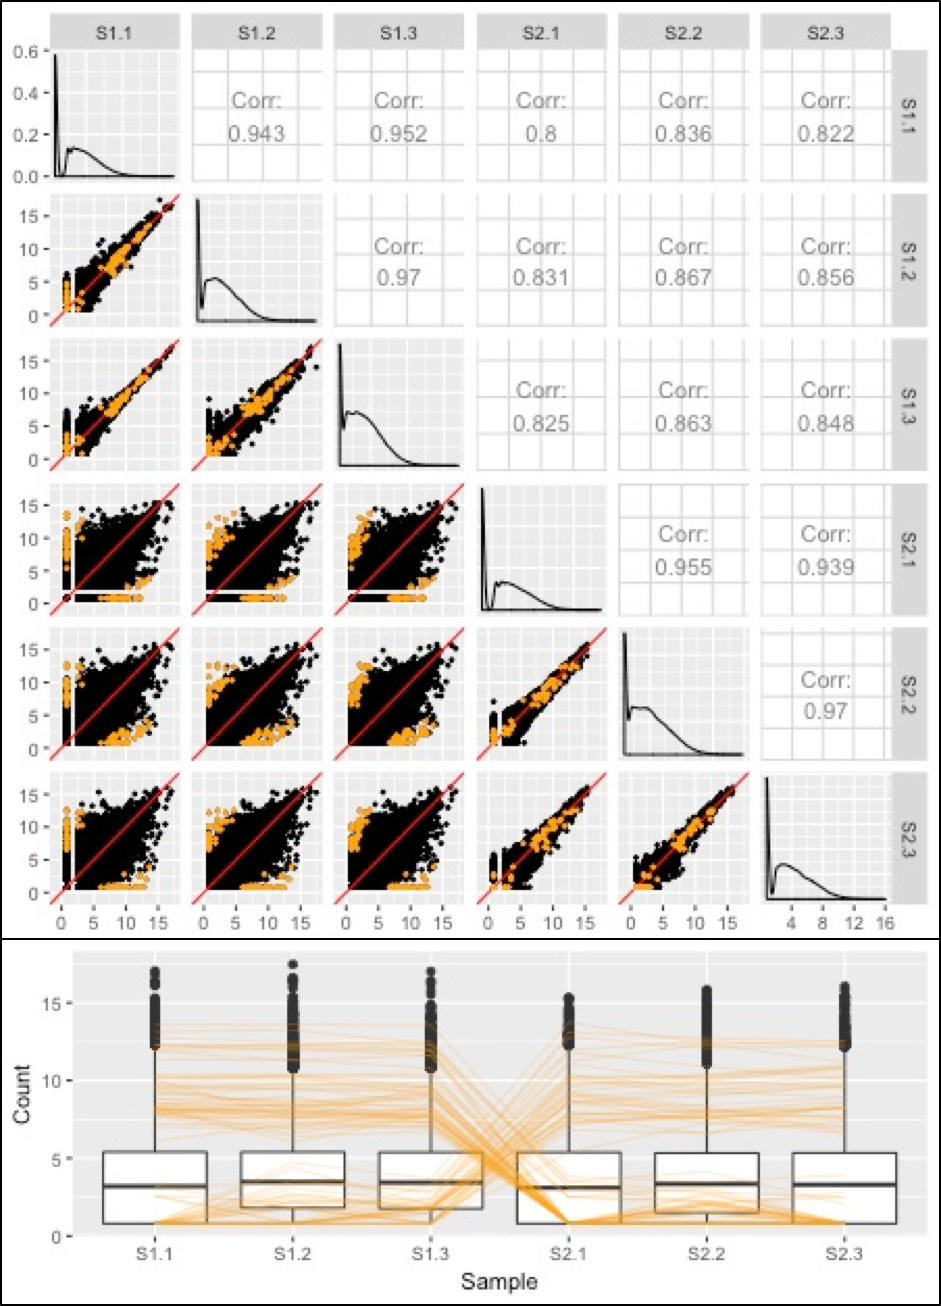
\includegraphics[width=7.5cm]{{/Users/lindz/JDSPaper/Bioinformatics/Pictures/SwitchSample/Switch12/NotSwitch/scatPCP}.png}}
\end{center}
\caption{Example of the expected structure of DEG calls (in orange) from an RNA-seq dataset. In the scatterplot matrix, DEGs should fall along the \textit{x=y} line for replicates and deviate from it for treatments. In the parallel coordinate plot, DEGs should show levelness between replicates and crosses between treatments. These two plotting types can be linked to quickly provide users multiple perspectives of their DEG calls.
\label{scatPCP}}
\end{figure}

\subsection{Assessing normalization with scatterplot matrices}
\label{s:Assessing normalization with scatterplot matrices}

There is still substantial discussion about the normalization of RNA-seq data, and the scatterplot matrix can be used to understand and assess various algorithms. To exemplify this point, we will use a publicly-available RNA-seq dataset on Saccharomyces cerevisiae (yeast) grown in YP-Glucose (YPD) (Risso, 2011). The data contained four cultures from independent libraries that were sequenced using two library preparation protocols and either one or two lanes in a total of three flow-cells (see Table~\ref{table:tableYeast} which is from Risso, 2011). This experimental design allowed researchers to examine various levels and combinations of technical effects (library preparation and protocol and flow cell) and biological effects (culture).

\begin{table}
\begin{tabular}{lrrr}
\Hline
Culture/Library prep. & \multicolumn{1}{c}{Library prep. protocol} &  \multicolumn{1}{c}{Growth condition} & \multicolumn{1}{c}{Flow-cell} \\ \hline
Y1 & Protocol 1 & YPD & 428R1 \\
Y1 & Protocol 1 & YPD & 4328B \\
Y2 & Protocol 1 & YPD & 428R1 \\
Y2 & Protocol 1 & YPD & 4328B \\
Y7 & Protocol 1 & YPD & 428R1 \\
Y7 & Protocol 1 & YPD & 4328B \\
Y4 & Protocol 2 & YPD & 61MKN \\
Y4 & Protocol 2 & YPD & 61MKN \\
\hline
\end{tabular}
\vspace{8mm}
\caption{We used this publicly-available RNA-seq dataset on Saccharomyces cerevisiae (yeast) growth because its design allows us to examine both technical effects (library preparation, flow cell, and lane) and biological effects (growth condition and culture). The authors used three growth conditions and ten cultures from independent colonies sequenced using two different library preparation protocols and either one or two lanes in a total of five flow-cells (Risso, 2011).}
\label{table:tableYeast}
\end{table}

The four cultures (Y1, Y2, Y4, and Y7) were treated as biological replicates for which differential expression was not expected. Hence, the authors could establish a false positive rate in relation to the number of DEGs called between these groups. They then demonstrated that within-lane regression alone was insufficient in effectively removing biases. Instead, aggressive corrections for both within-lane (GC-content and gene length) and between-lane (count distribution and sequencing depth) biases were needed to effectively reduce the false-positive rate of differential expression calls.

Figure~\ref{withinbtwn}A shows the scatterplot matrix of the read counts from the Y1 and Y4 treatments after within-lane normalization. As we stated earlier, we expect most genes to show similar expression between samples, except for the handful that are differentially expressed. However, it is immediately clear that the data still was not sufficiently normalized as the distribution of genes is not centered around the \textit{x=y} lines. In contrast, Figure~\ref{withinbtwn}B shows the scatterplot matrix of the read counts from the Y1 and Y4 treatments after \textit{both} within-lane and between-lane normalization, as was recommended by the authors due to its reduced false-positive rate. Indeed, the scatterplot matrix now follows the expected structure with most genes falling along the \textit{x=y} line with thicker deviations from it between treatment groups than between replicate groups.

Additionally, we can also confirm from Figure~\ref{withinbtwn}B that the read counts fall closer to the \textit{x=y} line between the Y4 replicates (bottom-right scatterplot) than between the Y1 replicates (top-left scatterplot). This is expected because the Y1 replicates had additional technical variability as they used two different flow cells, whereas the Y4 replicates were from the same flow cell. As such, the scatterplot matrix can also be used to quickly inspect patterns of biological and technical variability in the dataset.

\begin{figure}
\begin{center}
\centerline{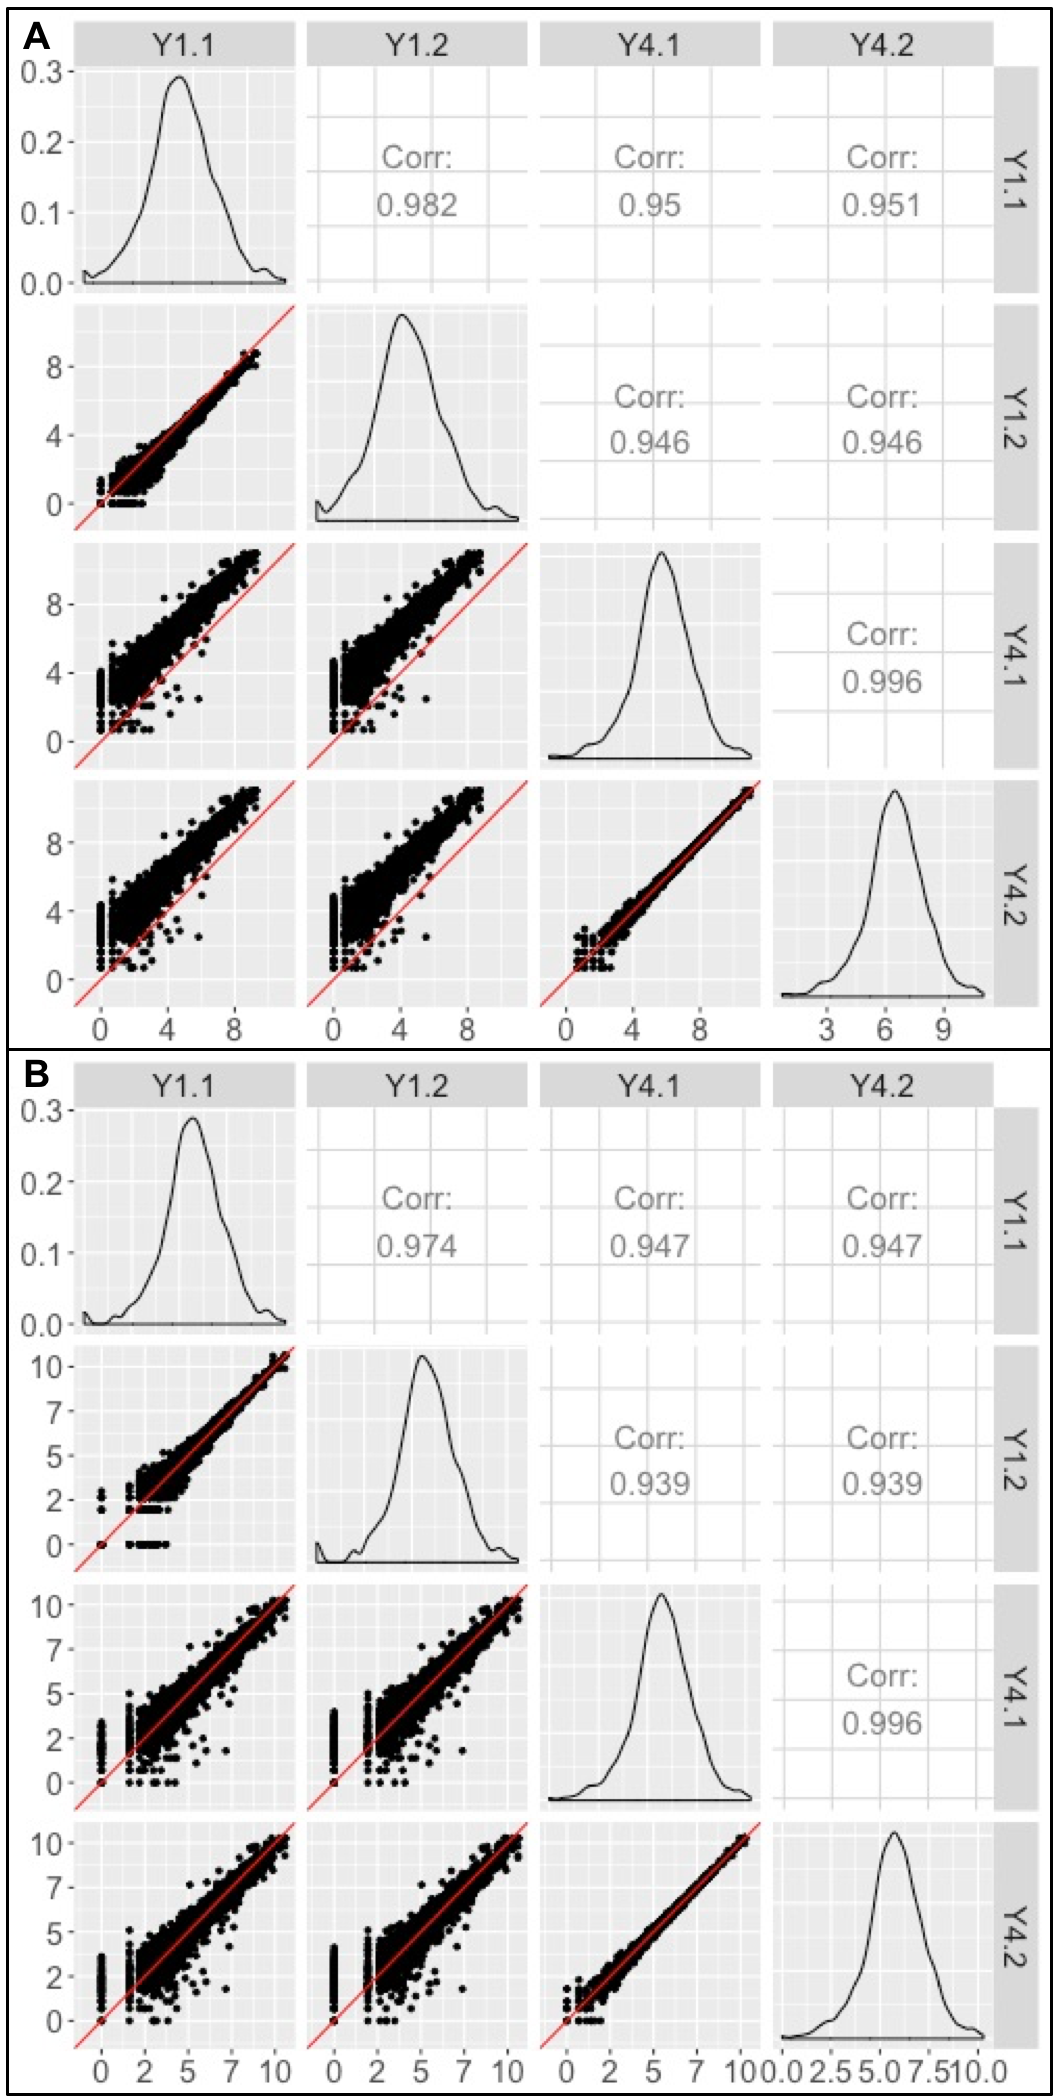
\includegraphics[width=7.5cm]{/Users/lindz/JDSPaper/Bioinformatics/Pictures/Figure4.png}}
\end{center}
\caption{The collective deviation of genes from the \textit{x=y} line instantly reveals that the RNA-seq dataset was not thoroughly normalized using within-lane normalization (subplot A). However, within-lane normalization followed by between-lane normalization sufficiently normalized the data (subplot B). The authors who developed these normalization methods showed that the later approach generated a lower false-positive DEG call rate in this dataset.
\label{withinbtwn}}
\end{figure}

\subsection{Checking for common errors with scatterplot matrices}
\label{s:Checking for common errors with scatterplot matrices}

Irreproducibility is prevalent in high-throughput biological studies. A study in Nature Genetics surveyed eighteen published microarray expression analyses and reported that only two were exactly reproducible (Ioannidis et al., 2009). The extent of the problem has spawned a field called ``forensic bioinformatics" whereby researchers attempt to reverse-engineer reported results back into the raw datasets simply to derive the methodologies used in published studies (Baggerly and Coombes, 2009).

Even though irreproducibility is merely cumbersome when it masks methods, it is unquestionably hazardous when it masks errors. With regards to personalized medicine, for example, obscured errors may cause well-intentioned researchers to present evidence for drugs that are ineffective or even harmful to patients (Baggerly and Coombes, 2009). Forensic bioinformaticians who have actively investigated common errors in high-throughput biological studies have concluded that the largeness of the data itself may hinder our ability to detect errors (Baggerly and Coombes, 2009). They also discovered that the most common errors are simple errors, such as mixing up sample labels (Baggerly and Coombes, 2009). Collectively, these findings suggest that simple errors can be difficult to detect using common practices in high-throughput studies.

Fortunately, scatterplot matrices are a simple tool to check for common errors like sample mislabeling. Figure~\ref{switchedScatMat} shows the resulting scatterplot matrix after we deliberately swapped the labels of the third replicate of the first treatment group (S1.3) with the first replicate of the second treatment group (S2.1) in the previously-mentioned cotyledon dataset. We can immediately see that, as expected, there are nine scatterplots with thicker distributions around the \textit{x=y} line and six scatterplots with thinner distributions around the \textit{x=y} line. However, we notice that a subset of these thick and thin scatterplots appear outside of their expected locations given the expected variability between treatments versus replicates. Rearranging the columns of the two samples that appear suspicious in Figure~\ref{switchedScatMat} would indeed lead us back to the clean-looking scatterplot matrix we saw in Figure~\ref{cotyIdeal}. We cannot detect this mislabeling problem as clearly and as convincingly with traditional plots, as can be verified with this dataset by comparing the boxplots and MDS plots before sample switching (left side of Figure~\ref{mdsSwitch}) and after sample switching (right side of Figure~\ref{mdsSwitch}). 

\begin{figure}
\begin{center}
\centerline{\fbox{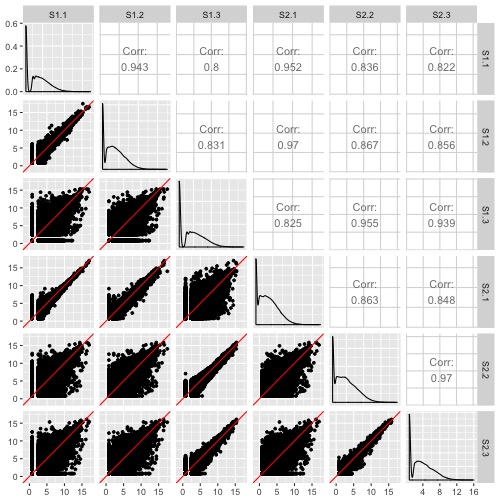
\includegraphics[width=7.5cm]{/Users/lindz/JDSPaper/Bioinformatics/Pictures/SwitchSample/Switch12/Switched/S1_S2_points.jpg}}}
\end{center}
\caption{As expected, this scatterplot matrix contains nine scatterplots with thicker distributions (should be treatment pairs) and six scatterplots with thinner distributions (should be replicate pairs). However, two samples appear to cause a subset of scatterplots to unexpectedly show thicker distributions between replicate pairs and thinner distributions between treatment pairs. If we switch the labels of these two suspicious samples (S1.3 and S2.1), the scatterplot matrix then displays the anticipated structure we saw in Figure~\ref{cotyIdeal}. At this point, we have evidence that these two samples may have been mislabeled, and we may wish to confirm this suspicion and correct it before continuing with the analysis.
\label{switchedScatMat}}
\end{figure}

\begin{figure}
\begin{center}
\centerline{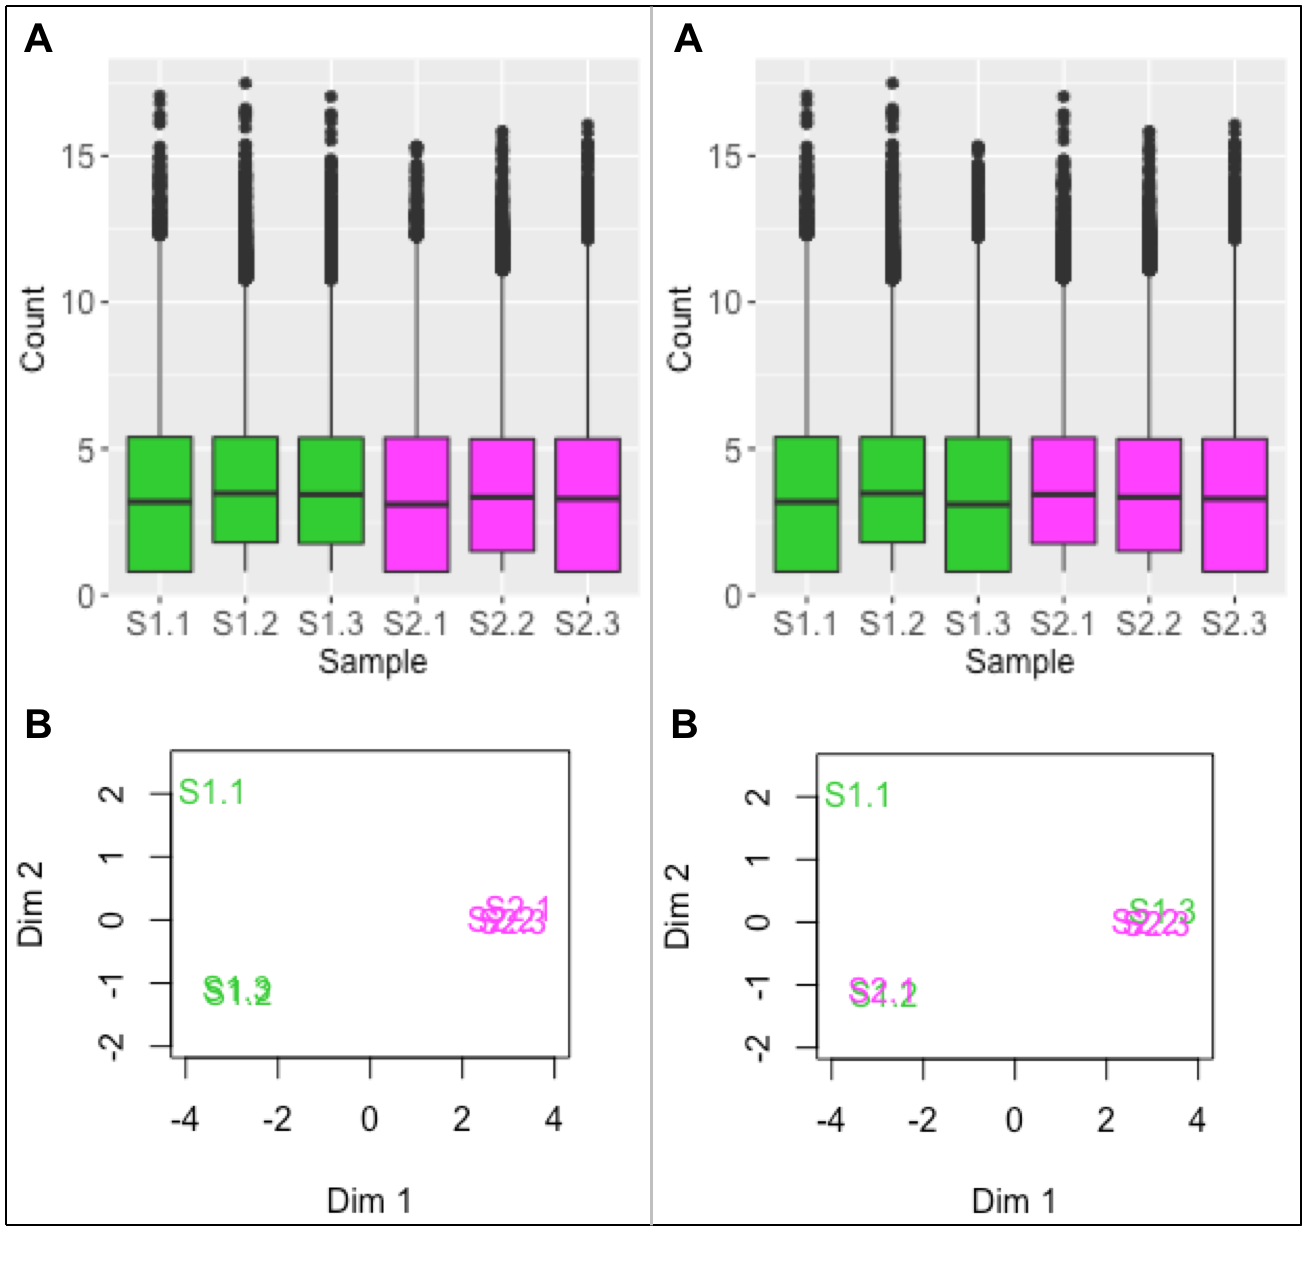
\includegraphics[width=7.5cm]{/Users/lindz/JDSPaper/Bioinformatics/Pictures/mdsSwitch.png}}
\end{center}
\caption{Boxplots and MDS plots are popular plotting tools for RNA-seq analysis. This figure shows these traditional plots applied to the cotyledon data before sample switching (left half) and after sample switching (right half). We cannot suspect from the right boxplot that samples S1.3 and S2.1 have been swapped (subplots A). This is because all six samples have similar five number summaries. For the MDS plots, we do see a cleaner separation of the two treatment groups across the first dimension in the left plot than in the right plot (subplots B). However, taking into account the second dimension, both MDS plots contain three clusters, with sample S1.1 appearing in its own cluster. Without seeing one distinct cluster for each of the two treatment groups, it is difficult to suspect that samples S1.3 and S2.1 have been swapped in the right MDS plot (subplots B). This is because we are not informed about variation at the gene level with the MDS plots like we were with the scatterplot matrix (Figure~\ref{switchedScatMat}).
\label{mdsSwitch}}
\end{figure}

\subsection{Finding unexpected patterns in scatterplot matrices}
\label{s:Finding unexpected patterns in scatterplot matrices}

Most popular RNA-seq plotting tools display summaries about the read counts, such as fold change summaries, principal component summaries, five number summaries, and dispersion summaries. In contrast to this trend, scatterplot matrices display the non-summarized read counts for all genes. This trait allows for geometric shapes and patterns relevant to the read count distribution to be readily visible in the scatterplot matrix.

An example of how geometric shapes in the scatterplot matrix can provide applicable information to researchers is shown in Figure~\ref{structure}. The dataset comes from an RNA-seq study conducted to identify gene expression responses in soybean leaves after exposure to iron-sufficient and iron-deficient soil conditions (Moran Lauter et al., 2014). After normalizing the data, we see the expected pattern of a scatterplot matrix in Figure~\ref{structure}, with more variation around the \textit{x=y} line between treatments than between replicates. 

However, one streak structure in the bottom right scatterplot stands out. A small subset of transcripts between replicates of the iron-sufficient group sharply deviates from the \textit{x=y} line. By interacting with the plot, we determined the identification of the five transcripts that deviated the most from the expected pattern, and searched for their putative functions. We discovered that these transcripts are reportedly involved in biotic and abiotic stress responses as well as the production of superoxides to combat microbial infections.

Discussion with the authors of the study revealed that a lab biologist documented accidentally tearing a leaf on one of these replicates. Hence, these transcripts that markedly deviate from the expected pattern in an otherwise well-controlled experiment might represent those that changed expression in relation to this incident. Even though the main motivation of the study had been to investigate the molecular underpinnings of iron metabolism, through our exploratory data analysis, we can derive a post-hoc hypothesis about what genes tentatively respond to leaf cutting. Of course, this would only serve as a hypothesis generator; conventional genetic studies and additional evidence would be needed to confirm any possible role these genes have on this biological activity. Regardless, we would not have observed this interesting structure or derived this post-hoc hypothesis from any models.

\begin{figure}
\begin{center}
\centerline{\fbox{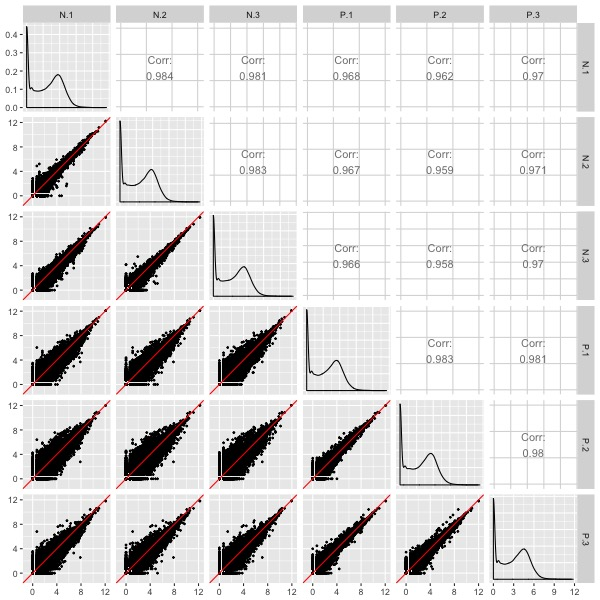
\includegraphics[width=7.5cm]{/Users/lindz/JDSPaper/Bioinformatics/Pictures/soybeanStreak/N_P_points.jpg}}}
\end{center}
\caption{Scatterplot matrix of RNA-seq read counts from soybean leaves after exposure to iron-sufficient (treatment group P) and iron-deficient (treatment group N) soil conditions. We observe the expected structure of treatment pairs showing larger variability around the \textit{x=y} line than replicate pairs. However, we notice a pronounced streak structure in the bottom-right scatterplot that compares two replicate samples from the iron-sufficient group. The genes in the streak structure have large read counts that deviate in a parallel fashion from the \textit{x=y} line. Through contacting the authors of this dataset, we discovered that a leaf on one of these samples was inadvertently torn and then documented as such during the experiment. Hence, the genes within this streak structure might represent those that responded to this leaf-tearing event, an observation discovered through the scatterplot matrix that could solidify into a post-hoc hypothesis.
\label{structure}}
\end{figure}

\section{Replicate point plots}
\label{s:repPoint}

We demonstrated how to view differentially expressed genes onto the Cartesian coordinates of the scatterplot matrix in Figure~\ref{scatPCP}. Unfortunately, this figure becomes limited when we investigate treatment groups that contain a large number of replicates because we then have too many small scatterplots for it to remain an effective visualization tool. Moreover, researchers could benefit from additional plotting tools that allow them to quickly verify individual differentially expressed genes returned from a model. As a result, we are developing a plot that allows users to visualize \textit{one} differentially expressed gene of interest onto the Cartesian coordinates of \textit{one} scatterplot matrix.

The ``replicate line plot" was developed by a group of researchers who demonstrated it could detect model scaling problems in microarray data (Cook et al., 2007). Unfortunately, this plot is only applicable on datasets where treatment groups contain exactly two replicates. The plot we now introduce is an extension of the ``replicate line plot" that can be applied to datasets with two or more replicates. We call this new plot a ``replicate point plot".

In the replicate point plot, each gene is plotted once for each possible combination of sample pairs between treatment groups. For example, there are nine ways to pair a sample from one treatment group with a sample from the other treatment group in the cotyledon dataset (S1.1 and S2.1, S1.1 and S2.2, S1.1 and S2.3, S1.2 and S2.1, S1.2 and S2.2, S1.2 and S2.3, and S1.3 and S2.1, S1.3 and S2.2, and S1.3 and S2.3). Hence, a given gene from this dataset is plotted as nine points in the replicate point plot. With 73,320 genes in this dataset, we would need to plot 659,880 points. This would reduce the speed of interactive functionality as well as cause overplotting problems. As a result, we again use hexagon bins to summarize this massive information (Figure~\ref{repDot} shows four example replicate point plots).

Once the background of hexagons has been drawn to give us a sense of the distribution of all treatment pair combinations for all genes, the user can superimpose the nine points of one gene of interest (colored orange in Figure~\ref{repDot}). Subplots A and B of Figure~\ref{repDot} show the replicate point plots for two example genes from the aforementioned cotyledon dataset, and subplots C and D of Figure~\ref{repDot} show the replicate point plots for two example genes from the cotyledon dataset after samples S1.3 and S2.1 have been swapped. Note that, in the examples in Figure~\ref{repDot}, the read counts of treatment pair combinations sometimes overlap, resulting in the appearance of less than nine orange points in a given replicate point plot.

\begin{figure}
\begin{center}
\centerline{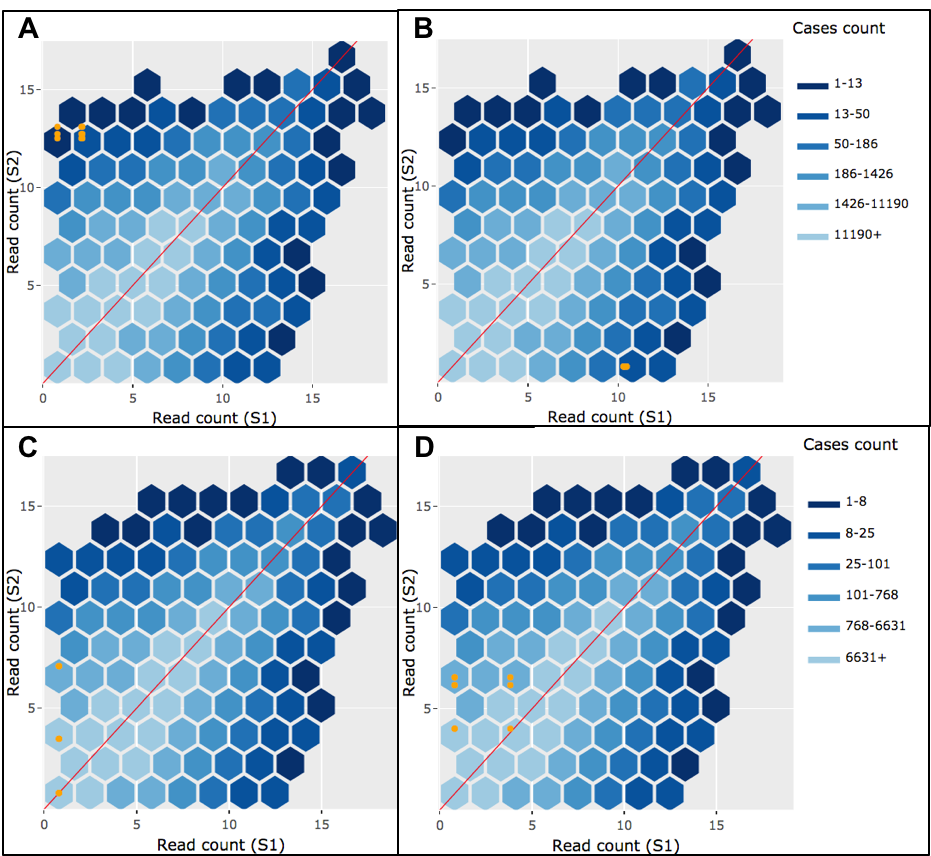
\includegraphics[width=7.5cm]{/Users/lindz/JDSPaper/Bioinformatics/Pictures/repDot.png}}
\end{center}
\caption{Subplots A and B each show a replicate point plot for a gene drawn from the ten genes with the lowest FDR values from the cotyledon data. In each case, the gene is overlaid as nine orange points (some of them overlap) showing the read count values for all nine combinations of treatment pairs. These two example genes show the pattern we expect from differentially expressed genes, having a large difference between treatments (distant from the \textit{x=y} line) and small difference between replicates (orange points close to each other). In contrast, subplots C and D each show a replicate point plot for a gene drawn from the ten genes with the lowest FDR values from the cotyledon data after samples S1.3 and S2.1 have been switched. These two example genes do not show the pattern we expect from differentially expressed genes, having a small difference between treatments (close to the \textit{x=y} line) and large difference between replicates (orange points far from each other). The interactive version of these plots confirms that the FDR values only reach significance for the cotyledon data before sample swapping, meaning the model and the visualizations are consistent. Hence, replicate point plots can be used to quickly sift through genes of interest and determine if the statistical outputs from the model sensibly match the visual findings.
\label{repDot}}
\end{figure}

The interactive replicate point plot for the cotyledon data (Figure~\ref{repDot}A and B) is available at https://rnaseqvisualization.shinyapps.io/repPoint, and the interactive replicate point plot for the cotyledon data after the samples were swapped (Figure~\ref{repDot}C and D) is available at https://rnaseqvisualization.shinyapps.io/repPointSwitch. As can be verified in the interactive version of the replicate point plot, users are provided several input fields that tailor the plot functionality. For instance, the user may wish to quickly scroll through differentially expressed genes one by one in the order of lowest to highest FDR values. Please read the ``About" tab in the interactive links for more information.

Figure~\ref{repDot}A and B show the static results of applying such settings to the cotyledon data. Each of these plots shows an example gene drawn from the ten genes with the lowest FDR values. For the case of Figure~\ref{repDot}A, the nine points of the gene are superimposed in a manner we would expect from a differently expressed gene: They are located far from the \textit{x=y} line (difference between treatments) and are close to each other (similarity between replicates). The points for the gene represented in Figure~\ref{repDot}B are also far from the \textit{x=y} line (difference between treatments) and are so close in proximity that they almost entirely overlay each other (precise similarity between replicates).

In contrast, Figure~\ref{repDot}C and D show the static results of applying such settings to the cotyledon data after swapping the S1.3 and S2.1 samples. Each of these plots shows an example gene drawn from the ten genes with the lowest FDR values. We expect this swap to cause the data to now produce unreliable results. Indeed, we can see this problem in Figure~\ref{repDot}C and D, as they contain orange points that are not far from the \textit{x=y} line and are not close to each other. This indicates that the genes with the lowest FDR values do not show the pattern we expect of differentially expressed genes. In this case, the results of the model match those from our visual exploratory analysis: As can be seen in the interactive graphic, none of the FDR values reached significance for the swapped cotyledon data.

Interestingly, we reach this same conclusion using parallel coordinate plots. In Figure~\ref{clusters}A, we took the 100 genes with the lowest FDR values from the cotyledon data and ran them through a hierarchical clustering algorithm with six clusters. Rather than plotting all 100 parallel coordinates onto a common background boxplot, we can reduce overplotting issues and see patterns more easily by separating with clustering. Nonetheless, we see that the six clusters all represent one of two expected patterns for differentially expressed genes: Each cluster either shows consistent high read counts for treatment S1 and consistent low read counts for treatment S2, or vice versa.

In contrast, Figure~\ref{clusters}B shows the result of taking the 100 genes with the lowest FDR values from the \textit{swapped} cotyledon data and running them through a hierarchical clustering algorithm with six clusters. Here, we see that the expression patterns do not fall into the two previously-mentioned expected patterns of differentially expressed genes. Instead, the difference between the treatment groups is suspiciously small and the difference between the replicates is suspiciously large. In addition, we may suspect that samples S1.3 and S2.1 were swapped: For example, the cluster with the largest number of genes (n=43) shows a pattern that would look more like differential gene expression if these two samples were reversed.

\begin{figure}
\begin{center}
\centerline{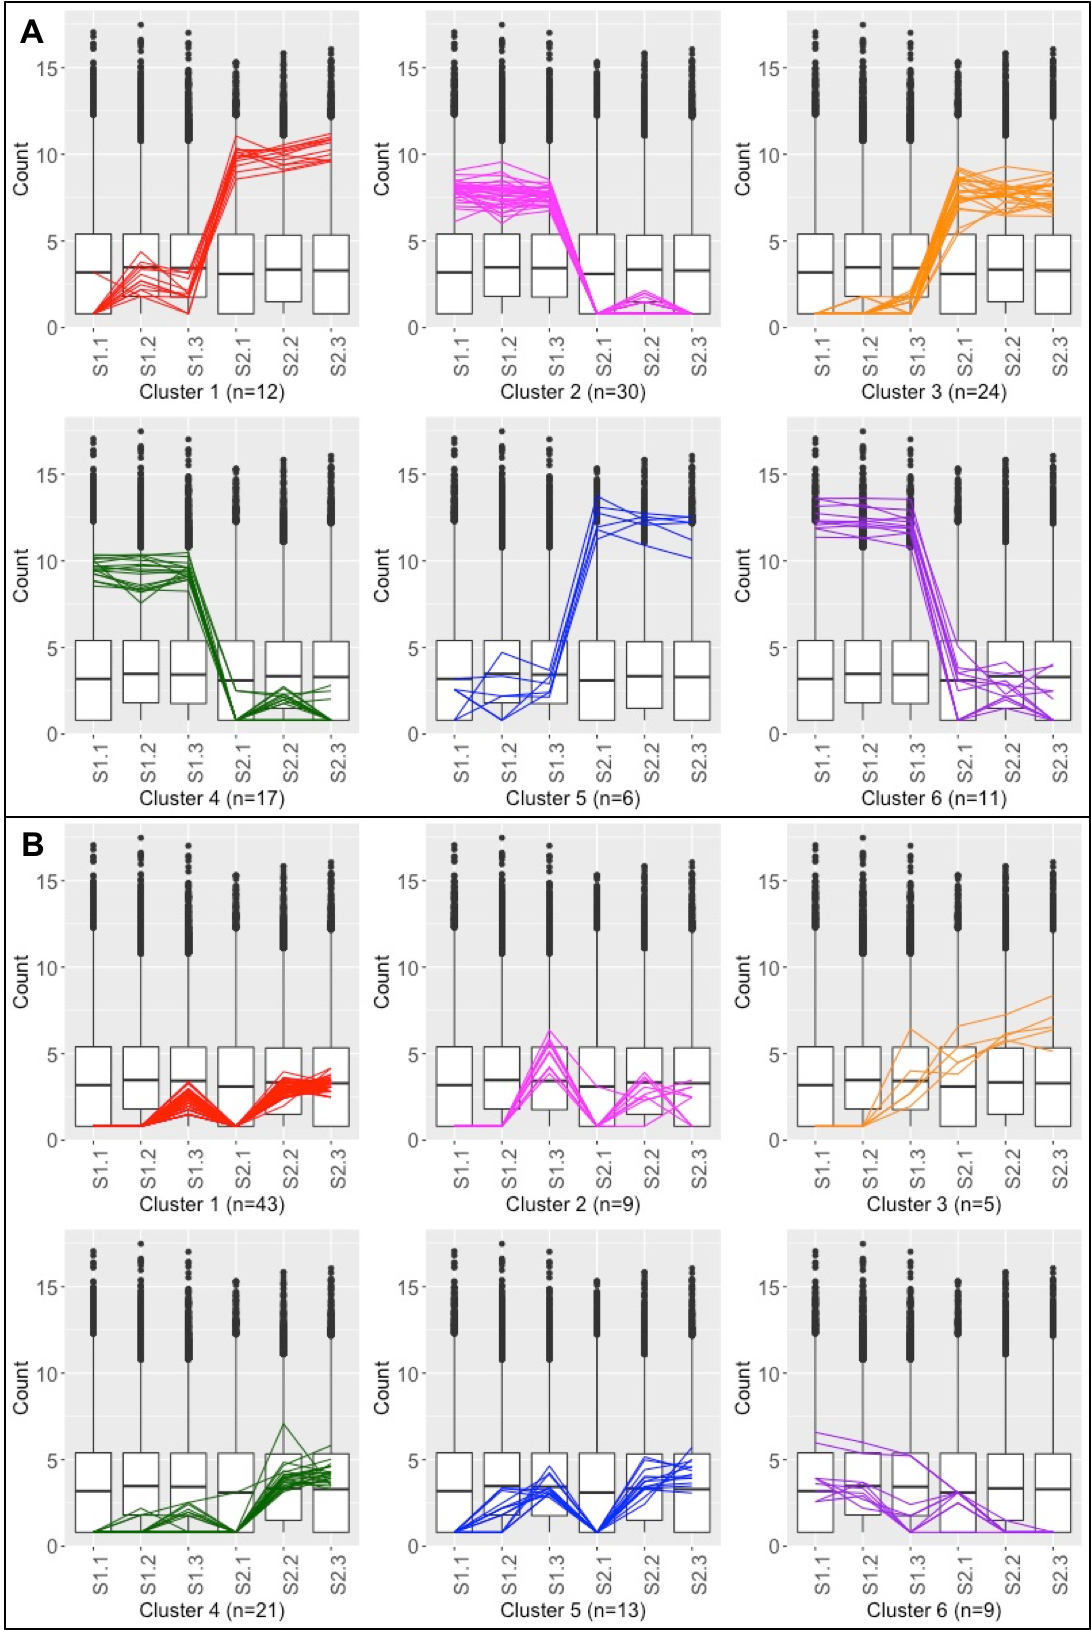
\includegraphics[width=7.5cm]{/Users/lindz/JDSPaper/clusters.png}}
\end{center}
\caption{Hierarchical clustering of the 100 genes with the lowest FDR values from the cotyledon dataset before (subplot A) and after (subplot B) swapping samples S1.3 and S2.1. The parallel coordinates show the expected structure of differentially expressed genes before sample swapping (subplot A), but not after sample swapping (subplot B).
\label{clusters}}
\end{figure}

\section{Discussion}
\label{s:discuss}

We have used real data to demonstrate that scatterplot matrices, parallel coordinate plots, and replicate point plots can help users check for normalization problems, catch common errors in the analysis pipeline, and confirm that the variation between replicates and treatments is as expected. We also show that these visual tools are useful for researchers to quickly investigate the list of differentially expressed genes that come out of a model and ensure which ones make sense. Similarly, in the case that no differentially expressed genes were returned, users can quickly investigate the list of genes with the lowest FDR values to ensure that the negative diagnosis of the model seems accurate. In addition, we demonstrated that our simple visualization tools can allow researchers to discover genes of interest that could not be obtained with models.

At this point, we aim to continue speeding up the interactive graphics, creating better color legends, extending the customisability of the graphics, and combining them into an easy-to-use \textsf{R} package for users. We plan to develop a clear and intuitive vignette for users to ensure them that rather than suggesting that they radically change their approach to RNA-seq analysis, we simply suggest that they incorporate these visual tools during their usual analysis pipeline to quickly check that the model assumptions and results are reasonable. We plan to include several real RNA-seq datasets in our \textsf{R} package and then demonstrate the syntax and value of our methods on these datasets in the vignette. Before publishing our \textsf{R} package, we will gather more examples using real RNA-seq data to show that these graphics can discover problems with or confirm proper use of popular RNA-seq analysis models.


%  The \backmatter command formats the subsequent headings so that they
%  are in the journal style.  Please keep this command in your document
%  in this position, right after the final section of the main part of 
%  the paper and right before the Acknowledgements, Supplementary Materials,
%  and References sections. 

\backmatter

%  This section is optional.  Here is where you will want to cite
%  grants, people who helped with the paper, etc.  But keep it short!


%  Here, we create the bibliographic entries manually, following the
%  journal style.  If you use this method or use natbib, PLEASE PAY
%  CAREFUL ATTENTION TO THE BIBLIOGRAPHIC STYLE IN A RECENT ISSUE OF
%  THE JOURNAL AND FOLLOW IT!  Failure to follow stylistic conventions
%  just lengthens the time spend copyediting your paper and hence its
%  position in the publication queue should it be accepted.

%  We greatly prefer that you incorporate the references for your
%  article into the body of the article as we have done here 
%  (you can use natbib or not as you choose) than use BiBTeX,
%  so that your article is self-contained in one file.
%  If you do use BiBTeX, please use the .bst file that comes with 
%  the distribution.  In this case, replace the thebibliography
%  environment below by 
%
%  \bibliographystyle{biom} 
% \bibliography{mybibilo.bib}

\begin{thebibliography}{}

\bibitem{ } Anders, S. and Huber, W. (2010). Differential expression analysis for sequence count data. \textit{Genome Biology} \textbf{11,} R106.

\bibitem{ } Anders, S., Reyes, A., and Huber, W. (2012). Detecting differential usage of exons from RNA-seq data. \textit{Genome Research} \textbf{22,} 2008–2017.

\bibitem{ } Baggerly, K.A. and Coombes, K.R. (2009). Deriving chemosensitivity from cell lines: Forensic bioinformatics and reproducible research in high-throughput biology. \textit{The Annals of Applied Statistics} \textbf{3,} 1309–1334.

\bibitem{ } Brown, A.V. and Hudson, K.A. (2015). Developmental profiling of gene expression in soybean trifoliate leaves and cotyledons. \textit{BMC Plant Biology} \textbf{15,} 169.

\bibitem{ } Bullard, J. H., Purdom, E., Hansen, K. D., and Dudoit, S. (2010). Evaluation of statistical methods for normalization and differential expression in mRNA-Seq experiments. \textit{BMC Bioinformatics} \textbf{11,} 94.

\bibitem{ } Cook, D., Hofmann, H., Lee, E.-K., Yang, H., Nikolau, B., and Wurtele, E. (2007). Exploring gene expression data, using plots. \textit{Journal of Data Science} \textbf{5,} 151-182.

\bibitem{ } Hansen, K.D., Brenner, S.E., and Dudoit, S. (2010). Biases in Illumina transcriptome sequencing caused by random hexamer priming. \textit{Nucleic Acids Research} \textbf{38,} e131.

\bibitem{ } Huber, W., Carey, V.J., Gentleman, R,, Anders, S,, Carlson, M., and Carvalho, B.S. (2015). Orchestrating high-throughput genomic analysis with Bioconductor. \textit{Nature Methods} \textbf{12,} 115-121.

\bibitem{ } Ioannidis, J.P., Allison, D.B., Ball, C.A., Coulibaly, I., Cui, X., Culhane, A.C., Falchi, M., Furlanello, C., Game, L., Jurman, G., Mangion, J., Mehta, T., Nitzberg, M., Page, G.P., Petretto, E. and van Noort, V. (2009). Repeatability of published microarray gene expression analyses. \textit{Nature Genetics} \textbf{41,} 149–155.

\bibitem{ } Law, C.W., Chen, Y., Shi, W., and Smyth, G.K. (2014). voom: Precision weights unlock linear model analysis tools for RNA-seq read counts. \textit{Genome Biology} \textbf{15,} R29.

\bibitem{ } Love, M.I., Huber, W., and Anders, S. (2014). Moderated estimation of fold change and dispersion for RNA-seq data with DESeq2. \textit{Genome Biology} \textbf{15,} 550.

\bibitem{ } Marini, F. (2017). pcaExplorer: Interactive visualization of RNA-seq data using a principal components approach. GitHub, Inc. https://github.com/federicomarini/pcaExplorer (accessed October 7, 2017).

\bibitem{ } Marioni, J.C., Mason, C.E., Mane, S.M., Stephens, M., and Gilad, Y. (2008). RNA-seq: An assessment of technical reproducibility and comparison with gene expression arrays. \textit{Genome Research} \textbf{18,} 1509–1517.

\bibitem{ } McIntyre, L.M., Lopiano, K.K., Morse, A.M., Amin, V., Oberg, A.L., Young, L.J., et al. (2011). RNAseq: Technical variability and sampling. \textit{BMC Genomics} \textbf{12,} 293.

\bibitem{ } Moran Lauter, A.N., Peiffer, G.A., Yin, T., Whitham, S.A., Cook, D., and Shoemaker, R.C. (2014). Identification of candidate genes involved in early iron deficiency chlorosis signaling in soybean (glycine max) roots and leaves. \textit{BMC Genomics} \textbf{15,} 1–25.

\bibitem{ } Morin, R., Bainbridge, M., Fejes, A., Hirst, M., Krzywinski, M., Pugh, T., et al. (2008). Profiling the HeLa S3 transcriptome using randomly primed cDNA and massively parallel short-read sequencing. \textit{Biotechniques} \textbf{45,} 81–94.

\bibitem{ } Oshlack, A., Robinson, M.D., and Young, M.D. (2010). From RNA-seq reads to differential expression results. \textit{Genome Biology} \textbf{11,} 220.

\bibitem{ } Pan, Q., Shai, O., Lee, L. J., Frey, B. J., and Blencowe, B. J. (2008). Deep surveying of alternative splicing complexity in the human transcriptome by high-throughput sequencing. \textit{Nature Genetics} \textbf{40,} 1413–1415.

\bibitem{ } Risso, D., Schwartz, K., Sherlock, G., Dudoit, S. (2011). GC-Content normalization for RNA-Seq data. \textit{BMC Bioinformatics} \textbf{12,} 480.

\bibitem{ } Ritchie, M.E., Phipson, B., Wu, D., Hu, Y., Law, C.W., Shi, W., and Smyth, G.K. (2015). Limma powers differential expression analyses for RNA-sequencing and microarray studies. \textit{Nucleic Acids Research} \textbf{43,} e47.

\bibitem{ } Robertson, G., Schein, J., Chiu, R., Corbett, R., Field, M., Jackman, S. D., et al. (2010). De novo assembly and analysis of RNA-seq data. \textit{Nature Methods} \textbf{7,} 909–912.

\bibitem{ } Robinson, M.D. and Oshlack, A. (2010). A scaling normalization method for differential expression analysis of RNA-seq data. \textit{Genome Biology} \textbf{11,} R25.

\bibitem{ } Robinson, M.D., McCarthy, D.J., and Smyth, G.K. (2010). edgeR: A Bioconductor package for differential expression analysis of digital gene expression data. \textit{Bioinformatics} \textbf{26,} 139–140.

\bibitem{ } Shneiderman, B. (2002). Inventing discovery tools: Combining information visualization with data mining. \textit{Information Visualization} \textbf{1,} 5-12.

\bibitem{ } Schurch, N.J., Schofield, P., Gierliński, M., Cole, C., Sherstnev, A., Singh, V., et al. (2016). How many biological replicates are needed in an RNA-seq experiment and which differential expression tool should you use? \textit{RNA} \textbf{22,} 839–851.

\bibitem{ } Shu, S., Ritchie, M.E., Law, C., and Lee, S. (2016). Glimma: Interactive HTML graphics. GitHub, Inc. https://github.com/Shians/Glimma/ (accessed October 7, 2017).

\bibitem{ } Trapnell, C., Hendrickson, D.G., Sauvageau, M., Goff, L., Rinn, J.L., and Pachter, L. (2013). Differential analysis of gene regulation at transcript resolution with RNA-seq. \textit{Nature Biotechnology} \textbf{31,} 46–53.

\bibitem{ } Trapnell, C., Roberts, A., Goff, L., Pertea, G., Kim, D., and Kelley D.R. (2012). Differential gene and transcript expression analysis of RNA-seq experiments with TopHat and Cufflinks. \textit{Nature Protocols} \textbf{7,} 562–578.

\bibitem{ } Wang, Z., Gerstein, M., and Snyder, M. (2009). RNA-Seq: A revolutionary tool for transcriptomics. \textit{Nature Reviews Genetics} \textbf{10,} 57–63.

\bibitem{ } Zhao, S., Fung-Leung, W.-P., Bittner, A., Ngo, K., and Liu, X. (2014). Comparison of RNA-Seq and microarray in transcriptome profiling of activated T cells. \textit{PLoS ONE} \textbf{9,} e78644.

\bibitem{ } Zhao, S., Fung-Leung, W.-P., Bittner, A., Ngo, K., and Liu, X. (2014). Comparison of RNA-Seq and microarray in transcriptome profiling of activated T cells. \textit{PLoS ONE} \textbf{9,} e78644.



\end{thebibliography}


\label{lastpage}

\end{document}